\documentclass{ctexart}
\bibliographystyle{plain}

\usepackage{graphicx}
\usepackage{amsmath}
\usepackage{amsfonts,amssymb}
\usepackage{algorithm}
\usepackage{algpseudocode}
\usepackage[export]{adjustbox}
\usepackage{subcaption}
\usepackage{url}
\graphicspath{{./img/}}

\begin{document}

\title{作业4\\Mandelbrot Set的生成和探索}
\author{张立言\\数学与应用数学 3210101207}
\maketitle

\begin{abstract}
Mandelbrot set是十分有趣的数学现象,它凭借神奇的图像特征而变得广为人知。本报告利用了C++和Bitmap库生成Mandelbrot set的图像并作出一些处理和探索,并且引申了tricorn set的图像。

\end{abstract}
\section{引言}
Mandelbrot set,中文名又叫做曼德博集合。它是由复平面上组成分形的点组成的一种集合,最早在1978年由Robert W.Brooks和Peter Matelski定义并提出。后来在1980年由Benoit Mandelbrot作出了可视化处理并且最终广为人知\cite{aa}。它的神奇之处在于,在图形的“边界”处不断进行放大总会有更多的细节显示出来。关于它的一些性质,许多数学家作出了探索,并且得出了一些结论,而也有很多猜想尚未得到证明,例如其局部联通性质(local connectedness)和某些特殊点的自相似性(self-similarity)。我们利用一些简单的数学结论辅助完成本次可视化Mandelbrot set的工作。

\section{问题的背景介绍}
我们不必要关心Mandelbrot set的拓扑性质,但可以利用一些简单的结论辅助我们优化我们的可视化处理。绘制Mandelbrot set的图像的主要目的是练习掌握和使用Linux系统工作的技巧。
\section{数学理论}
Mandelbrot set的通常定义如下:
使得复平面上的迭代方程
\begin{equation}
z_{n+1}=z_n^2+c \label{iteq}
\end{equation}
在初始值$z_0=0$时进行迭代能够最终收敛的所有$c$的集合。其中,$c \in \mathbb{C}$.
下面给出一些关于该集合的一些基本的性质:
在实轴上,Mandelbrot set为严格的闭区间$[-2,\frac{1}{4}]$.拓扑学家证明了它的连通性。接下来介绍一些对于我们编写程序很有用的结论:
\subsection{Theorem 1}
\textbf{若$c\in M$,则$|c|\le 2$}

\textit{Proof}{}\cite{a} 假设$|c|>2$,则$|z_1|=|c|,|z_1|>2$\par
当$n=2$时,
$$|z_2|=|z_1^2+c|\le |c^2|-|c|$$
由$|c|>2$可知
$$|c|^2-|c|>|c|$$
从而$|z_2|>|c|$\par
假设$|z_n|>|c|$成立,则$|z_n|>2$,
$$|z_{n+1}|=|z_n^2+c|\le |z_n|^2-|c|$$
又因为$|z_n|>2$,从而
$$|z_{n+1}|>|z_n|^2-|z_n|>|z_n|$$
可知$|z_n|$递增,从而$|z_n|>|z_1|>2$.假如$|z_n|$不发散,由于它递增,从而收敛至某一常数$a$.于是由$|z_{n+1}|\le |z_n|^2-|c|$取极限可得$a\le a^2-|c|\Rightarrow a^2-a=a(a-1)\le a\le |c|$,矛盾,故而$|z_n|$发散。
\subsection{Theorem 2}
\textbf{若$c \in M$则$|z_n|\le 2$}\par
限于篇幅,该定理的证明略去。

这个定理是我们判定收敛的一个重要的定理,我们可以避免一般的收敛判定繁琐的部分,使得编程难度降低和程序运行的效率提高。而且,由定理的证明过程,我们发现当迭代方程\ref{iteq}中的$z_n$项换成其共轭不会影响以上两个定理的成立。这允许了我们探索一种新的迭代,其图形又叫做Tricorn set.
\section{算法}
生成Mandelbrot set图像的伪代码如下:
\begin{algorithm}
\caption{Generating image of Mandelbrot set}
\label{alg1}
\begin{algorithmic}
\Require Max iteration time and criterion of convergence
\State Getting the value of c
\State Initrialize the $z_0$ $z \gets 0$
\While{$|z| \le 2$ and iteration time < max iteration time}
\State $z \gets z^2 + c$
\EndWhile
\If{Iteration time = max iteration time}
\State c point converges, draw color
\Else{} c point diverges, draw color
\EndIf
\end{algorithmic}
\end{algorithm}
我们作出一些细微的处理,让程序更加好用。
\subsection{Color our set}
在老师所给出的程序的基础上,我们可以调整着色的参数,让图案变得更加具有美感。

我们以进行迭代的次数为依据,迭代次数越少,说明其“收敛程度”越高,根据这个参数调整RGB参数,可以呈现出多种颜色,同时也利于我们观察图像的特征。而由于收敛的点执行循环的次数为最大迭代次数,这使得我们判定的收敛的c值可以呈现出同一个颜色,从而呈现出Mandelbrot set的大致形状。

itn的意义也使得我们免去了判定的麻烦而直接进行调色。为了让颜色变化更明显,我采用了非线性的变化方式,但是保持了RGB第一个参数(蓝色)始终为255,这确定了颜色的基调为蓝色。类似的,我们可以设置更多样的颜色变化,这些并不困难,我们可以通过尝试找出更美观的变化。
\subsection{Zooming into the set}
我们在老师给出的程序中可以进行放大,但我们难以确定放大位置。引入了itn参数之后,我们可以很容易解决这个问题。虽然Mandelbrot set很大,我们无法从它的本身入手,但我们可以考虑不收敛但是很“靠近”收敛的地方,从那里放大,我们可以观察到更细致的局部。限于代码水平和知识有限,我只对代码作出一些小的修改,使其可以定位“边界”并且生成不断放大的图像。
\subsection{Max iteration time and accuracy}
随着迭代次数的增加,我们会很自然的认为图像的精度会增加。这是明显的,在实验过程中,我们也可以简单验证一下这种性质。
\section{数值算例}
\subsection{Varied colors}
\begin{figure}[H]

\begin{subfigure}{0.5\textwidth}
	\centering
	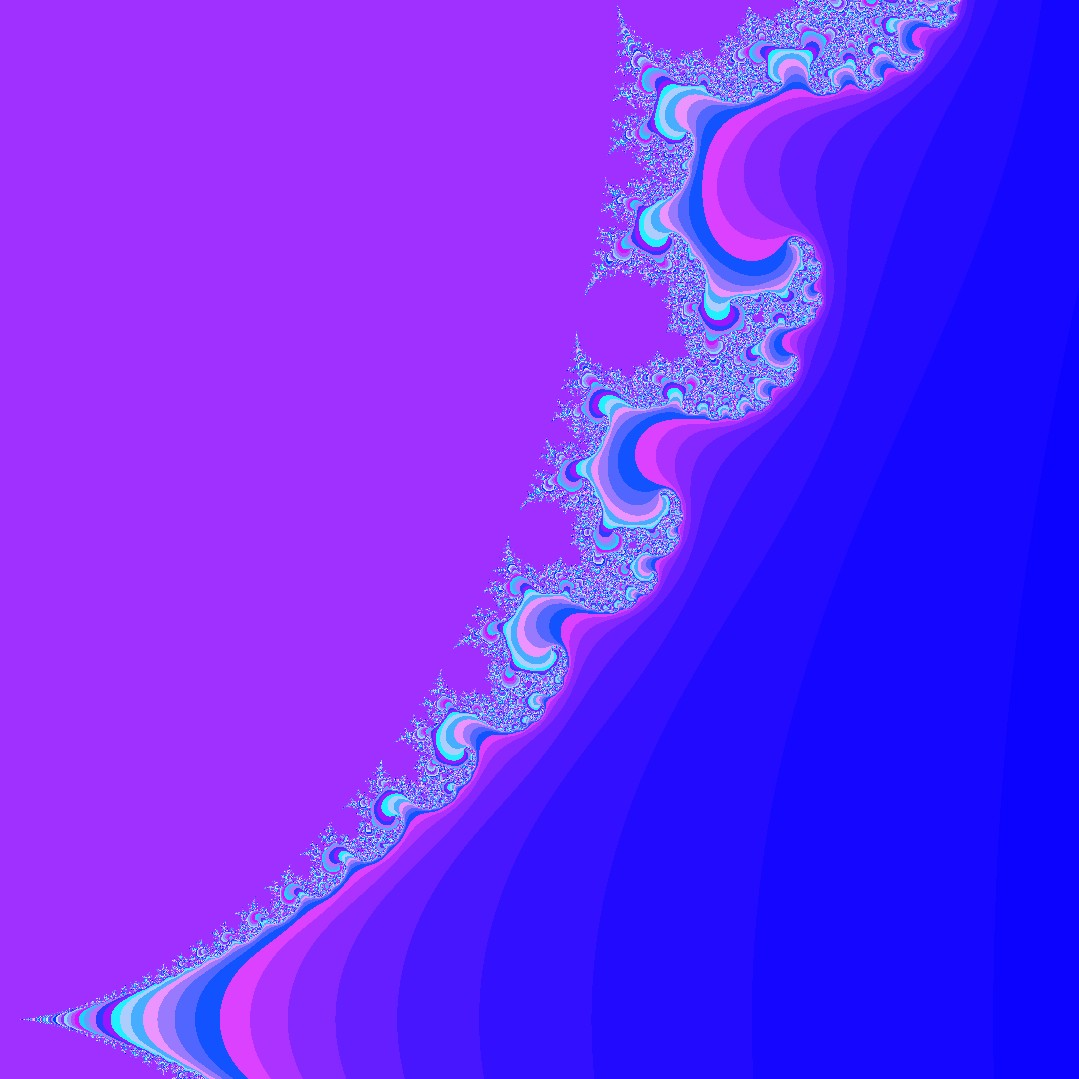
\includegraphics[width=0.9\linewidth]{blue.jpg}
	\caption{Blue theme}
\end{subfigure}
\begin{subfigure}{0.5\textwidth}
	\centering
	
\includegraphics[width=0.9\linewidth]{red1.jpg}
	\caption{Red theme}
\end{subfigure}
\caption{A zoom-in at around (0.3,0.1)}
\end{figure}
上面的颜色我分别调整蓝色和红色的数值为255,其他两个参数按照一个迭代次数按四次幂函数表达式的一个变化。不使用其他非多项式的数学表达式(考虑到系统性能)。
\subsection{Zooming and accuracy}
下面的一系列图片都是由程序自动寻找合适点(即靠近“边界”的地方),并且依次放大的结果。其中每次放大倍数均为4倍。
\begin{figure}[H]
\begin{subfigure}{0.16\textwidth}
	\centering
	\includegraphics[width=\linewidth]{run0.bmp}
\end{subfigure}
\begin{subfigure}{0.16\textwidth}
	\centering
	\includegraphics[width=\linewidth]{run1.bmp}
\end{subfigure}
\begin{subfigure}{0.16\textwidth}
	\centering
	\includegraphics[width=\linewidth]{run2.bmp}
\end{subfigure}
\begin{subfigure}{0.16\textwidth}
	\centering
	\includegraphics[width=\linewidth]{run3.bmp}
\end{subfigure}
\begin{subfigure}{0.16\textwidth}
	\centering
	\includegraphics[width=\linewidth]{run4.bmp}
\end{subfigure}
\begin{subfigure}{0.16\textwidth}
	\centering
	\includegraphics[width=\linewidth]{run5.bmp}
\end{subfigure}
\begin{subfigure}{0.16\textwidth}
	\centering
	\includegraphics[width=\linewidth]{run6.bmp}
\end{subfigure}
\begin{subfigure}{0.16\textwidth}
	\centering
	\includegraphics[width=\linewidth]{run7.bmp}
\end{subfigure}
\begin{subfigure}{0.16\textwidth}
	\centering
	\includegraphics[width=\linewidth]{run8.bmp}
\end{subfigure}
\begin{subfigure}{0.16\textwidth}
	\centering
	\includegraphics[width=\linewidth]{run9.bmp}
\end{subfigure}
\caption{A zoom-in image series with max iteration = 500}

\end{figure}
对比一下,我们设置最大迭代次数为100的时候,有如下系列图。
\begin{figure}[H]
\begin{subfigure}{0.3\textwidth}
	\centering
	\includegraphics[width=\linewidth]{5.bmp}
\end{subfigure}
\begin{subfigure}{0.3\textwidth}
	\centering
	\includegraphics[width=\linewidth]{6.bmp}
\end{subfigure}
\begin{subfigure}{0.3\textwidth}
	\centering
	\includegraphics[width=\linewidth]{7.bmp}
\end{subfigure}

\begin{subfigure}{0.3\textwidth}
	\centering
	\includegraphics[width=\linewidth]{8.bmp}
\end{subfigure}
\begin{subfigure}{0.3\textwidth}
	\centering
	\includegraphics[width=\linewidth]{9.bmp}
\end{subfigure}
\begin{subfigure}{0.3\textwidth}
	\centering
	\includegraphics[width=\linewidth]{10.bmp}
\end{subfigure}
\caption{A zoom-in image series with max iteration = 100}
\end{figure}
从上面的放大过程我们可以看到,最大迭代次数越大,放大后的图像越显得平滑。数学上,随着其趋于无穷大,呈现出的结果是计算机难以模拟的。
\subsection{结论}
根据程序的运行,我们可以得出多彩的画面,具有独特的美感。同时,我们也可以简单地从观察的角度的出Mandelbrot set的一些几何特征。这次的探索使我加深了对于程序各个技能的理解。
\bibliography{hmwk4}

\end{document}
